\chapter{研究基础与相关技术}

近年来,深度学习一直是计算机领域乃至多学科交叉应用领域的研究热点,不仅在计算机视觉方向有着广泛的应用,在光学、材料和航空航天等领域也出现了相关研究。尤其对于大数据应用场景,基于深度学习的方法已经成为重要的数据挖掘手段。
对于气动优化乃至整个CFD领域而言,深度学习方法在此领域获得发展并取得成功只是时间问题。
为了便于阐述本课题工作,本章首先定义了本课题要解决的问题,即明确利用深度学习方法和技术要解决的问题和要达到的效果;
其次介绍了CFD相关的基础理论,主要包括建立在宏观层次的Navier-Stokes(N-S)方程和介观层次的格子Boltzmann方法(Lattice Boltzmann Methods,LBM);最后介绍了四种与本文工作紧密相关的深度神经网络和图神经网络模型。

\section{研究问题定义}
利用传统CFD方法对流体问题(包括气动优化问题)进行研究的流程如图\ref{fig:cfdflow}所示。
\begin{figure}[htp]
	\centering
	%\includegraphics[width=0.42\textwidth]{data/MLP.pdf}
	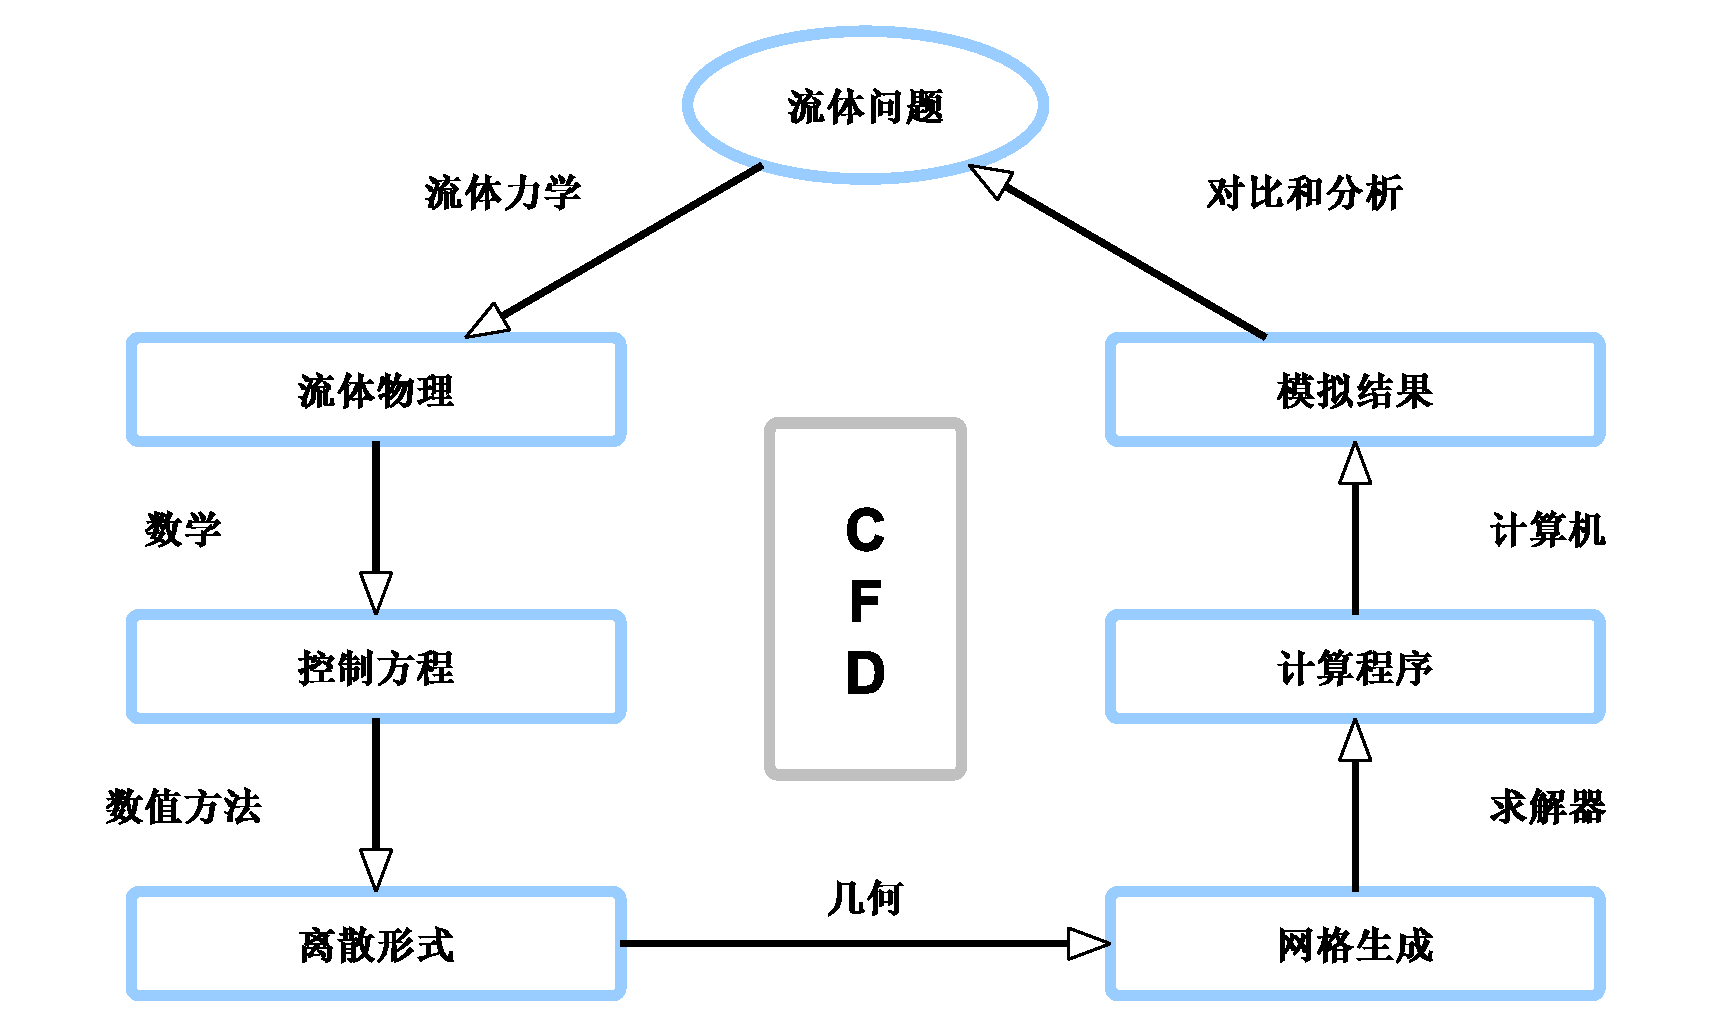
\includegraphics[width=0.92\textwidth]{figures/cfdflow.pdf}
	\caption{利用传统CFD方法研究和解决流体问题的流程示意图}
	\label{fig:cfdflow}
\end{figure}


首先利用流体力学知识对流体问题进行分析并建立物理模型;
根据流体运动遵循的基本规律利用数学方法推导出流体流动的控制方程,
宏观层面上有粘性流动的Navier-Stokes方程和无粘流动的欧拉方程;
针对特定的流体问题,明确其物理基础和假设,简化控制方程、确定边界条件和初始条件。
由于CFD方法是利用数值计算对流体流动进行模拟,必须利用数值方法对时间和空间进行离散,
以便进行迭代计算求解。对空间的离散方法包括有限差分方法\cite{Forsythe1960Finite},有限元方法\cite{Strang1974An}和有限体积方法\cite{Eymard2000The};
对时间的离散通常包括适用于定常流体问题求解的显示方法和适用于非定常问题的求解的隐式方法。
确定离散形式之后,需要进行网络生成,继而选择合适的CFD求解器,依据初始条件和边界条件对求解器的参数进行设置,
最后利用计算机进行迭代计算至模拟结果收敛。



这种全阶CFD模拟往往耗时较长,难以满足全面、快速的设计空间探索需求。
针对二维稳态流动问题,本文使用深度学习方法构建了两种气动优化模型以加速CFD模拟进程,提升气动优化效率,图\ref{fig:cfd_dnnflow}展示了这两种模型的工作流程。

\begin{figure}[htp]
	\centering
	%\includegraphics[width=0.42\textwidth]{data/MLP.pdf}
	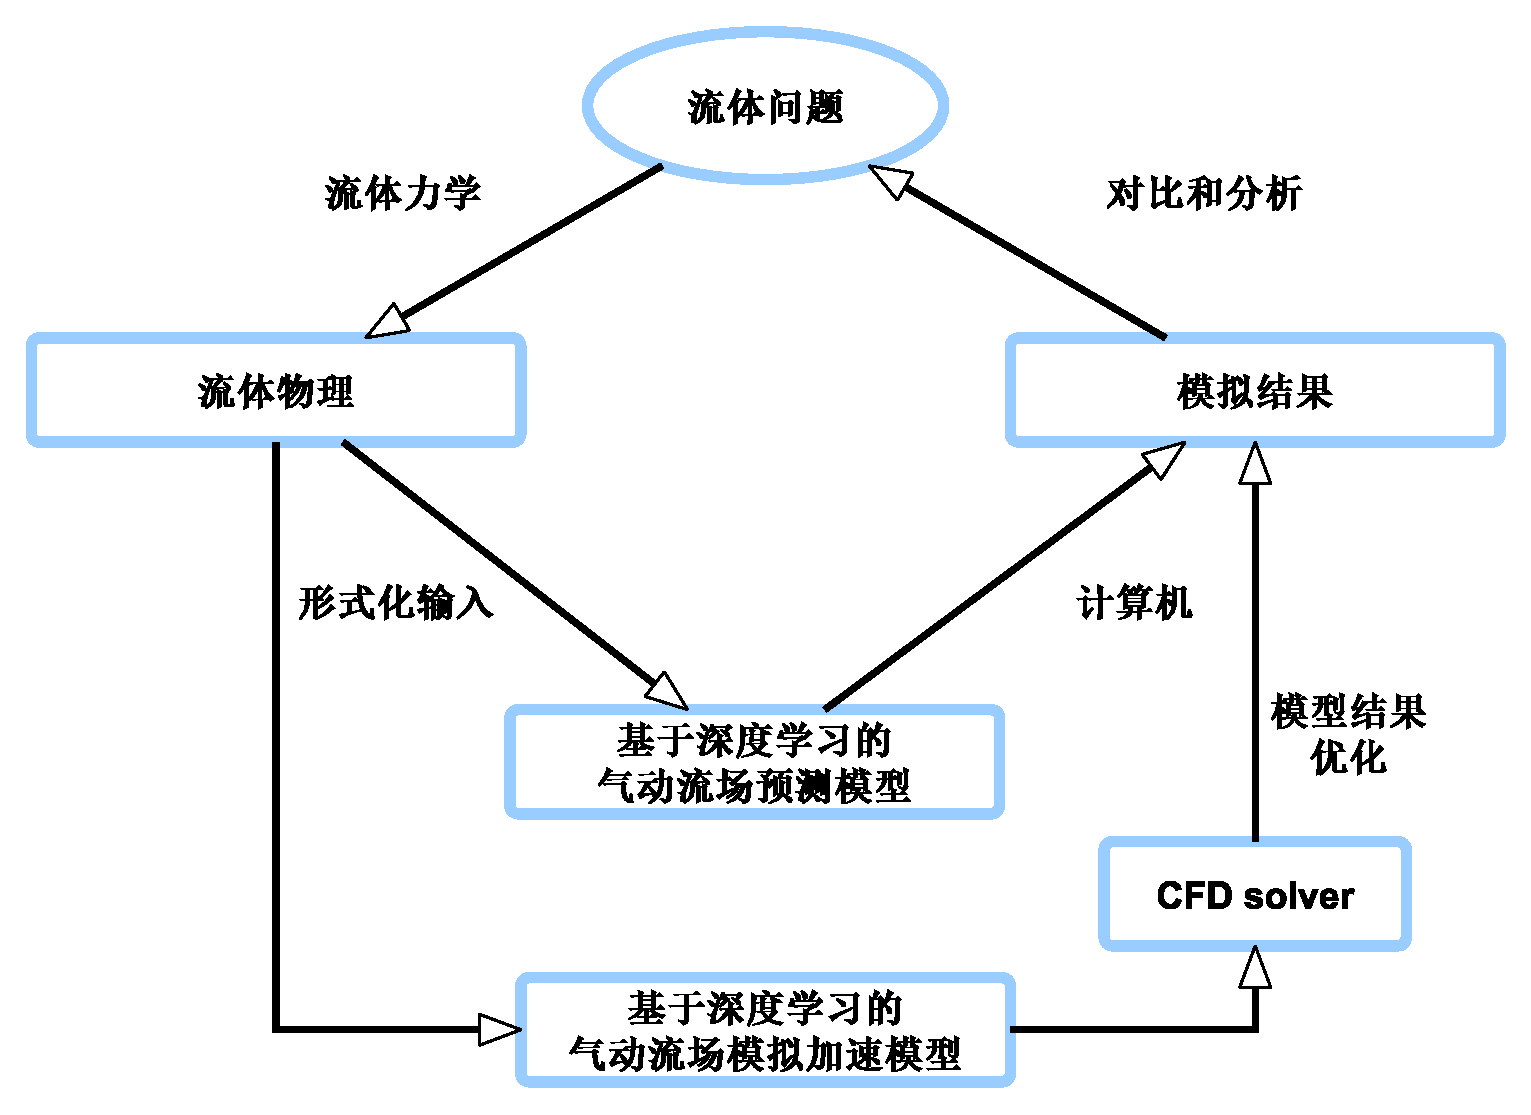
\includegraphics[width=0.92\textwidth]{figures/cfd_dnnflow.pdf}
	\caption{基于深度学习的气动优化模型工作流程示意图}
	\label{fig:cfd_dnnflow}
\end{figure}

在气动流场预测模型中,将边界条件和几何外形形式化为适合神经网络训练的输入,
利用深度学习方法构建端到端的预测模型,通过神经网络正向推理过程,得到对应的气动流场预测结果;
气动流场模拟加速模型的流程与气动流场预测模型类似,不同之处在于模型训练完成后,将深度学习模型的结果输入到CFD求解器中,为CFD求解过程提供一个更加接近收敛状态的初场,从而达到减少迭代计算量、加速模拟的效果。



\section{计算流体动力学基础理论}
计算流体力学方法可根据对液体和气体在不同尺度上动力学规律的描述分为宏观、介观和微观三类。
宏观尺度上,假设流体连续地充满整个空间,流体被假设为连续介质并且满足质量守恒、动量守恒以及能量守恒;在数学上利用欧拉方程组或N-S方程组对流体运动进行描述;在数值计算上,通过各种离散方法控制方程离散成各种代数方程。
介观(分子自由程)尺度上,将流体看成离散的流体粒子并在数学上利用统计力学方程对流体的运动进行描述;基于物理规律的定义流体粒子运动机制,计算得到与物理规律相符的数值结果。
微观尺度上,不再假设流体介质为连续的,通过对每一个分子的运动进行模拟计算并在采用不同的方式进行统计平均,获得流体的宏观运动规律。因为要对每一个分子的运动进行模拟计算,微观层面的方法往往需要消耗大量的计算资源。
根据与本文研究内容的相关性,本节重点介基于介观尺度的绍格子Boltzmann方法和基于宏观尺度的雷诺平均N-S方程。



\subsection{格子Boltzmann方法的基本原理}

\subsubsection{BGK模型}
Boltzmann方程的基本思想是宏观系统中每一个微观分子的运动都遵循力学规律,
利用统计学方法求解粒子状态分布即可得到系统的宏观变量。
基于以上思想引出方程的三大假设:
\begin{itemize}
	\item[(1)] 不考虑3个及3个以上分子碰撞,将分子碰撞限定在两个分子之间的碰撞;
	\item[(2)] 每个分子的速度不受其他分子的影响;
	\item[(3)] 局部碰撞不受外界作用力影响。	
\end{itemize}

定义速度分布函数$f$是位置矢量$\vec{r}$,速度矢量$\vec{\xi}$以及时间$t$的函数,则有:
\begin{equation}n=\int f(\vec{r}, \vec{\xi}, t) d \xi\end{equation}
\noindent n即为t时刻,$\vec{r}$处单位体积内的分子数。
根据假设,速度分布函数$f$可分子的运动和分子的碰撞两项改变。
假设在没有碰撞的情况,m和$m \vec{a}$分别是分子质量作用在每个分子上的外力。
如果在时间间隔$d t$内无碰撞,则分子位置由$\vec{r}$变为$\vec{r}+d \vec{r}$,
速度变为$\vec{\xi}+\vec{a} d t$,则原t时刻,在$d \vec{r} d \vec{\xi}$中的分子移动至$\vec{r}+d \vec{r}$,$\vec{\xi}+\vec{a} d t$的$d \vec{r} d \vec{\xi}$中,即有
\begin{equation}f(\vec{r}+d \vec{r}, \vec{\xi}+\vec{a} d t, t+d t) d \vec{r} d \vec{\xi}=f(\vec{r}, \vec{\xi}, t) d \vec{r} d \vec{\xi}\end{equation}

\noindent 在$(\vec{r}, \vec{\xi}, t)$处进行Taylor展开,化简得分子的运动对f的影响:

\begin{equation}
\label{运动}
\left(\frac{\partial f}{\partial t}\right)_{\text {运动 }}=-\vec{\xi} \cdot \frac{\partial f}{\partial \vec{r}}-\vec{a} \cdot \frac{\partial f}{\partial \vec{\xi}}\end{equation}

\noindent 考虑分子间的碰撞,应用刚体碰撞模型,根据碰撞前后动量守恒和能量守恒可得碰撞对速度分布函数的影响:

\begin{equation}
\label{碰撞}
\left(\frac{\partial f_{1}}{\partial t}\right)_{\text {碰撞 }}=\iint\left(f_{1}^{\prime} f_{2}^{\prime}-f_{1} f_{2}\right) d_{D}^{2}|\vec{g}| \cos \theta d \Omega d \vec{\xi}_{2}\end{equation}

\noindent  其中$\vec{g} =  f_{1} - f_{2}$, $f_{1}$,$f_{2}$为碰撞前分子速度,$f_{1}^{\prime}$,$f_{2}^{\prime}$为碰撞后分子速度;$d_{D}$是分子直径,
$d \Omega$表示球面微元在前一个分子的固定角。

综合公式\ref{运动}和\ref{碰撞}有:
\begin{equation}\left(\frac{\partial f}{\partial t}\right)=\left(\frac{\partial f}{\partial t}\right)_{\text {运动 }}+\left(\frac{\partial f}{\partial t}\right)_{\text {碰撞 }}\end{equation}

\noindent 化简即有:
\begin{equation}
\label{Boltzmann方程}
\left(\frac{\partial f}{\partial t}\right)+\vec{\xi} \cdot \frac{\partial f}{\partial \vec{r}}+\vec{a} \cdot \frac{\partial f}{\partial \vec{\xi}}=\iint\left(f_{1}^{\prime} f_{2}^{\prime}-f_{1} f_{2}\right) d_{D}^{2}|\vec{g}| \cos \theta d \Omega d \vec{\xi}_{1}\end{equation}

由于碰撞项计算涉及复杂的非线性积分,所以玻尔兹曼方程难以求解。因此BGK近似模型提出使用算子$\Omega_{f}$替代方程\ref{Boltzmann方程}右边碰撞项。
可以简单假设碰撞使f趋于稳定分布$f^{e q}$。
假设变化率与$\left(f^{eq}-f\right)$成正比且比例系数为$\nu$,即碰撞频率即弛豫时间的导数${1}/{\tau_{0}}$,则玻尔兹曼方程简化为:

\begin{equation}\left(\frac{\partial f}{\partial t}\right)+\vec{\xi} \cdot \frac{\partial f}{\partial \vec{r}}+\vec{a} \cdot \frac{\partial f}{\partial \vec{\xi}}=v\left[f^{e q}(\vec{r}, \vec{\xi}, t)-f(\vec{r}, \vec{\xi}, t)\right]\end{equation}

\noindent 等式右边即为线性算子$\Omega_{f}$。

\subsubsection{格子Boltzmann方程}
将BGK方程在速度和时空上离散可得LBM方程。
尽管微观粒子热运动时刻存在,粒子的速度矢量分布是连续函数,但单个粒子的运动对系统宏观量几乎没有影响。
因此可对分子速度进行有限离散,$\left\{\overrightarrow{e_{0}}, \vec{e}_{1}, \ldots, \overrightarrow{e_{N}}\right\}$,N表示速度总数。
对速度分布函数进行N维离散有$\left\{f_{0}, f_{1}, \ldots, f_{N}\right\}$,
其中$f_{\alpha}=f_{\alpha}\left(\vec{r}, \overrightarrow{e_{\alpha}}, t\right)$,
$\alpha=0,1, \ldots, N$。于是可得离散的Boltzmann方程:

\begin{equation}
\label{速度离散}
\frac{\partial f_{\alpha}}{\partial t}+\overrightarrow{e_{\alpha}} \cdot \nabla f_{\alpha}=-\frac{1}{\tau_{0}}\left(f_{\alpha}-f_{\alpha}^{e q}\right)+F_{\alpha}\end{equation}

\noindent 其中$f_{\alpha}^{e q}$分子局部平衡分布;$F_{\alpha}$是外力项。
对速度离散后的玻尔兹曼方程进一步进行时间离散和空间离散,对公式\ref{速度离散}积分,采用矩形法对公式右边项进行逼近有:

\begin{equation}
\label{LBM方程}
f_{\alpha}\left(\vec{r}+\overrightarrow{e_{\alpha}} \delta_{t}, t+\delta_{t}\right)-f_{\alpha}(\vec{r}, t)=-\frac{1}{\tau}\left[f_{\alpha}(\vec{r}, t)-f_{\alpha}^{e q}(\vec{r}, t)\right]+\delta_{t} F_{\alpha}(\vec{r}, t)\end{equation}

方程\ref{LBM方程}即为格子玻尔兹曼方程。
DnQm模型\cite{Y1992Lattice}是格子玻尔兹曼方程基本模型,n表示空间维数,m表示速度的类型,图\ref{fig:dnqm}给出了常见的D2Q9模型和D3Q19模型的示意图。


\begin{figure}[htb]
	\centering
	\subfloat[D2Q9]{\label{fig:d2q9}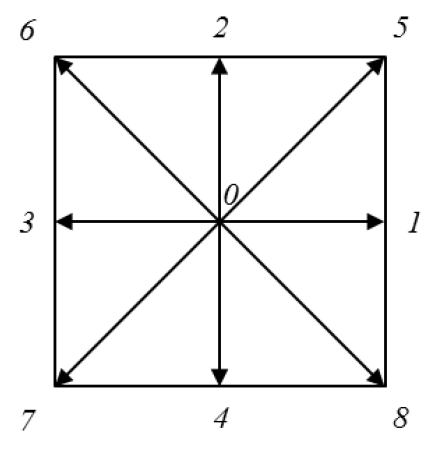
\includegraphics[width=0.35\textwidth]{figures/d2q9.png}} \qquad
	\subfloat[D3Q19]{\label{fig:d3q19}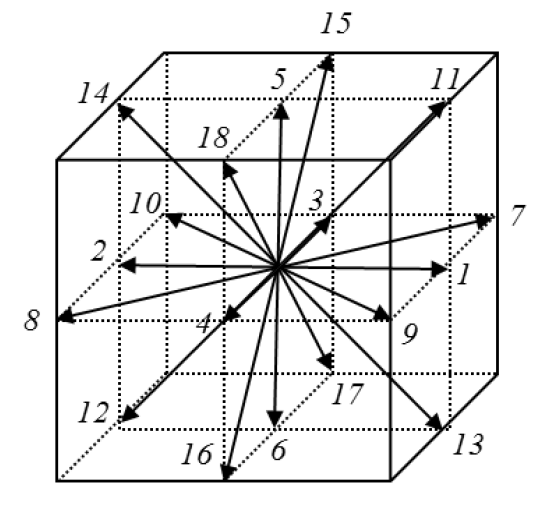
\includegraphics[width=0.38\textwidth]{figures/d3q19.png}} 
	\caption{D2Q9模型和D3Q19模型速度离散示意图}
	\label{fig:dnqm}
\end{figure}

\noindent D2Q9模型适用于二维流动问题,将速度根据大小和方向的不同分为了9类;
D3Q19模型适用于三维流动问题,速度离散也更加复杂,将速度根据大小和方向的不同分为了19类。

LBM方法相对于宏观方法具有精度高的特点,与传统方法相比,对流项(碰撞项)是线性的,算法简单;由于粒子的运动只有碰撞和迁移,LBM方法编程容易;
此外,LBM运算具有局部性,每个粒子只与周围相邻粒子有关,局部运算可同步进行,适合并行计算。
因为以上优点,LBM方法在CFD领域应用广泛,利用深度学习技术提升LBM方法的模拟效率具有重要意义。


\subsection{雷诺平均N-S(RANS)方程}
流体流动一般由三大基本定律来控制,基于这三个基本的物理学定理构建的流动模型,将导出一组控制方程来描述流体的运动。
流体的流动状态和流速紧密相关,随着流速的增加,流体进过层流、过度流和湍流等状态,
各个状态流体中流体运动的不规则度逐渐增加。

湍流运动过程十分复杂,在数学上表现出极高的非线性,使用数值模拟方法通常难以解决湍流问题。
尽管湍流流动能被N-S方程精确描述,但该方程求解时间、经济成本巨大。

目前在CFD工程应用领域,通常使用直接数值模拟、大涡模拟和雷诺平均( Reynold average Navier-Stokes,RANS)方法解决湍流问题。
其中DNS和LES对网格精细度要求较高,在工程应用上还处于尚不成熟的阶段。
为了在精度和效率上满足实际工程需要,研究者提出了基于时均理论的雷诺平均N-S模型,RANS在工程上应用也最多。
对于本文研究的稳态不可压流动,在笛卡尔坐标系下有,连续性方程:

\begin{equation}
\label{连续性方程}
\frac{\partial \rho}{\partial t}+\frac{\partial(\rho u)}{\partial x}+\frac{\partial(\rho v)}{\partial y}+\frac{\partial(\rho w)}{\partial z}=0\end{equation}

\noindent 对动量方程采用二阶迎风对流格式离散:


\begin{equation}\begin{array}{c}
\label{动量方程}
u \frac{\partial u}{\partial x}+v \frac{\partial u}{\partial y}+w \frac{\partial u}{\partial z}=-\frac{1}{\rho} \frac{\partial p}{\partial x}+\frac{\mu}{\rho} \nabla^{2} u \\
u \frac{\partial v}{\partial x}+v \frac{\partial v}{\partial y}+w \frac{\partial v}{\partial z}=-\frac{1}{\rho} \frac{\partial p}{\partial y}+\frac{\mu}{\rho} \nabla^{2} v \\
u \frac{\partial v}{\partial x}+v \frac{\partial w}{\partial y}+w \frac{\partial w}{\partial z}=-\frac{1}{\rho} \frac{\partial p}{\partial z}+\frac{\mu}{\rho} \nabla^{2} w
\end{array}
\end{equation}


\noindent 对方程\ref{连续性方程}和\ref{动量方程}进行雷诺平均有:
\begin{equation}\frac{\partial \rho}{\partial t}+\frac{\partial}{\partial x_{i}}\left(\rho \bar{u}_{i}\right)=0\end{equation}

\begin{equation}\frac{\partial}{\partial t}\left(\rho \bar{u}_{i}\right)+\frac{\partial}{\partial x_{i}}\left(\rho \bar{u}_{j} \bar{u}_{i}\right)=-\frac{\partial \bar{p}}{\partial x_{i}}+\frac{\partial \bar{\sigma}_{i j}}{\partial x_{j}}+\frac{\partial}{\partial x_{j}}\left(-\rho \bar{u}_{i}^{\prime} \bar{u}_{j}^{\prime}\right)\end{equation}

\noindent 其中$\bar{u}_{i}$为雷诺平均速度分量,$\rho$为密度,$p$为压强,$\bar{u}_{i}^{\prime}$平均脉动速度,$\partial \bar{\sigma}_{i j}$为应力张量分量。


使用RANS方法对对湍流问题进行处理会引入雷诺应力项,该未知量会导致方程组无法求解,
因此需要构建符合物理规律和相关约束条件的湍流模型封闭方程组
此外,在进行雷诺平均的过程中损失了部分流动细节,引入湍流模型对于找回这些细节十分必要。
对于RANS湍流模拟,根据布辛尼斯克\cite{schmitt2007boussinesq}假设,粘性系数由层流部分和湍流部分构成,
即$\nu=\nu_{L}+\nu_{T}$,其中$\nu_{L}$是层流运动粘性系数(laminar kinematic viscosity), $\nu_{T}$是湍流运动粘性系数(eddy-viscosity variable),由湍流模型方程计算得到。

常用的湍流模型可根据所采用的微分方程数进行分类为:零方程模型、一方程模型、两方程模型、四方程模型、七方程模型等\cite{1998A}。本文使用的常用于航空航天领域的一方程Spalart-Allmaras(SA)湍流模型\cite{SAequation}。
SA模型认为在自由剪切流中能量和信息由大尺度流动流向小尺度流动,涡粘系数只有产生项和扩散项,所以满足以下基本运输方程:

\begin{equation}
\begin{split}
\frac{D F}{D t}= & \frac{\partial F}{\partial t}+(u \cdot \nabla) F \\ = & {Diffusion} + {Production} - {Destruction}
\end{split}
\end{equation}

\noindent 其中$F$外力,\textit{diffusion}是扩散项,\textit{production}是产生项,\textit{destruction}是损失项。
对于湍流运动粘性系数$\nu_{T}$应用该运输方程有:

\begin{equation}\label{SA_equo}
\begin{split}
\frac{D \nu_{T}}{D t}=& \frac{1}{\sigma}\left[\nabla \cdot((\nu_{L}+\nu_{T}) \nabla \nu_{T})+c_{b 2}(\nabla \nu_{T})^{2}\right] +c_{b 1} \tilde{S} \nu_{T} - \\ &c_{w 1} f_{w}\left[\frac{\nu_{T}}{d}\right]^{2}
\end{split}
\end{equation}

\noindent 其中$\sigma$普朗特数,$c_{b 1}$和$c_{b 2}$为闭合常数,$d$表示到壁面的最短距离。
$\tilde{S}$可以通过$d$和速度$u$计算得到,
$f_{w}$是一个关于$\tilde{S}$和$\nu_{T}$无量纲函数,用于解决在边界层外部损失项收敛慢的问题。

至今大多数湍流模型缺少通用性,只适用于特定场景,这也直接导致了RANS缺少普适性。
本文首先基于特定流场条件,模拟生成流场数据集,然后利用深度学习方法从大量流场数据学习流场运动规律,
最后得到能够进行快速精准流场预测的代替模型。


\section{深度学习相关模型介绍}
深度学习2006年提出以来,深度学习相关理论和技术以及获得了长足的发展,常见的深度学习模型有深度信念网络\cite{深度信念网络},自动编码器\cite{Bengio2013Representation},卷积神经网络\cite{Lecun1998Gradient},递归神经网络\cite{Williams2014A},生成对抗网络\cite{GAN}等。
此外,深度学习在与强化学习、图网络结合方面也取得突破性进展,比较前沿的研究领域有深度强化学习\cite{Deepreinforcementlearning}和图神经网络\cite{2016Semi}等。
深度学习的快速发展为解决气动优化提供了新的思路和方法,
利用深度学习方法提升气动优化效率的核心思想是基于神经网络构建从输入到输出的映射函数,
从而代替或者加速CFD求解器的迭代计算过程,
不同于常规的图像分类任务,深度神经网络需要在大量数据中学习到从给定输入到对应输出的表示方法。

针对流场数据中的欧式空间数据,经过类比分析,我们发现图像处理中的image-to-image\cite{DBLP:conf/miccai/RonnebergerFB15,DBLP:conf/cvpr/LongSD15,isola2017image,CycleGAN2017,DBLP:conf/cvpr/AmodioK19}的转换方法尤其适用于气动优化场景。
对于非欧式空间数据,引入了基于图神经网络的架构进行模型训练。
本节重点介绍三类用于图像回归任务的深度神经网络和图神经网络中的图卷积网络。
关于深度学习的其他基础理论知识包括网络基础结构单元,损失函数,优化算法等,可参见文献\cite{dnnsurvey}。

\subsection{卷积自编码网络}
卷积自编码网络(Convolutional Autoencoders)是自编码网络\cite{Bengio2013Representation}的变体。
自编码网络及其变体都有类似的网络结构:编码器和解码器。
传统的自编码器是一种无监督学习算法,数据没有标签,
输入数据$X$经过编码器处理得到输入数据的特征表示z,编码结果经过解码器得到输出$X^{\prime}$,具体过程可以表示为:
\begin{equation}
z=g(X ; \phi) 
\vspace{-0.2cm}
\end{equation}
\begin{equation}
X^{\prime}=f(z ; \theta)
\end{equation}
其中$g(\bullet ; \phi)$和$f(\bullet ; \theta)$分别表示编码器和解码器,$\phi$和$\theta$是相应的参数。

损失函数一般可以定义为输入$X$和输出$X^{\prime}$的最小均方误差(Mean Squared Error,MSE):
\begin{equation}
Loss_{MSE} = \min _{\phi, \theta}\left\|X-X^{\prime}\right\|_{2}^{2}
\end{equation}

一般而言,z的维度远小于输入$X$的维度,网络通过这样编码和解码的方式,实现对输入数据的降维且尽量不损失数据信息。

但是传统的自编码器在处理图片格式数据时,由于采用了全连接操作进行数据堆叠,忽略了图像中的空间关系,会导致信息大量丢失。
为了克服这一缺点,卷积自编码网络采用卷积层来构造自编码器。
图\ref{fig:CAE}是卷积自编码网络的示意图,深色部分代表编码器,通常由卷积层和池化层构成,卷积层负责信息提取,池化层负责空域下采样;
浅色部分代表解码器,由卷积层和上采样层构成,有时也利用逆卷积操作替代卷积和上采样操作进行原始信息的复原。

\begin{figure}[htp]
	\centering
	%\includegraphics[width=0.42\textwidth]{data/MLP.pdf}
	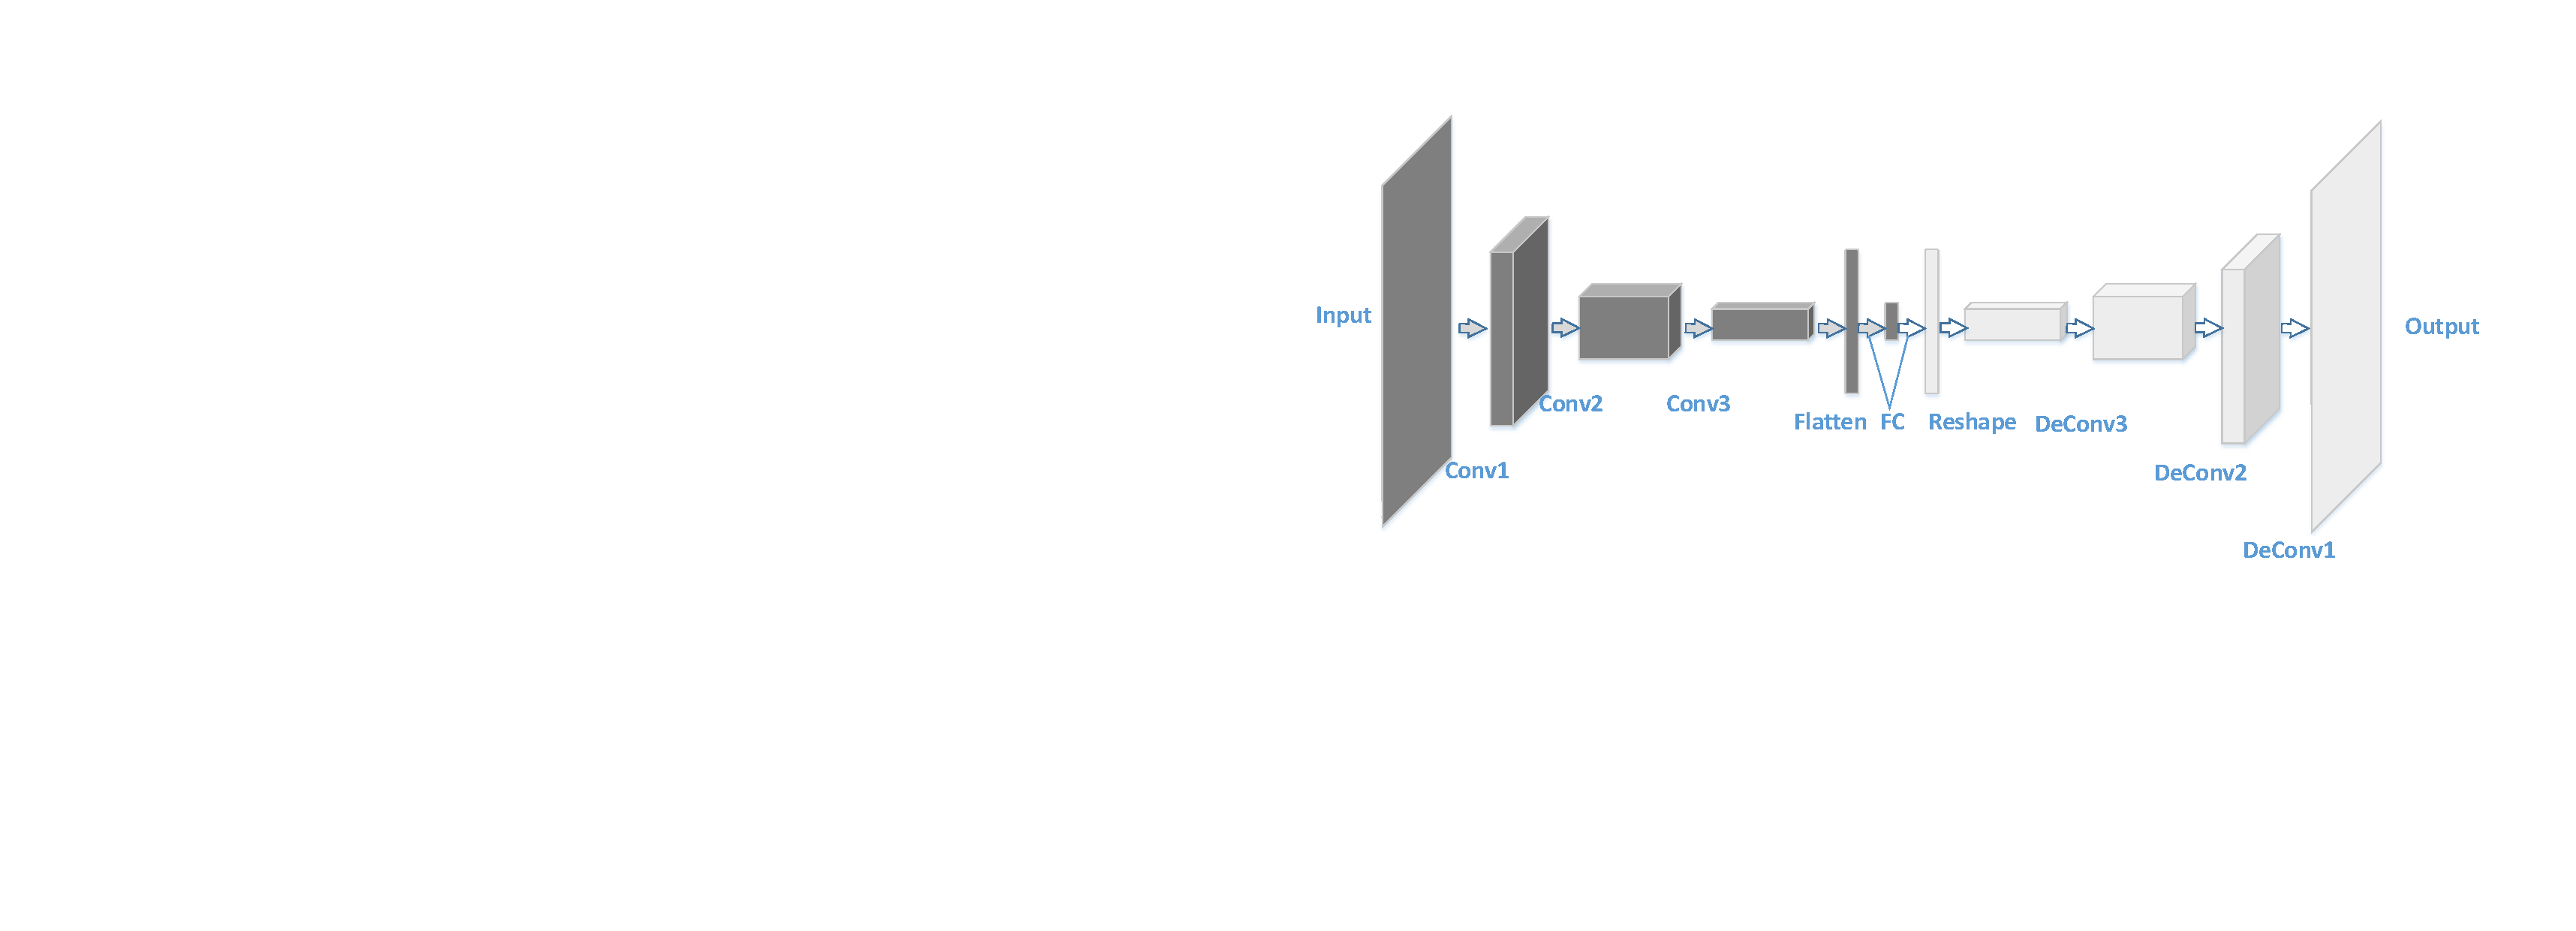
\includegraphics[width=0.92\textwidth]{figures/CAE.pdf}
	\caption{卷积自编码网络示意图}
	\label{fig:CAE}
\end{figure}

逆卷积操作原理如图\ref{fig:conv_dconv}所示,逆卷积操作可以看出是常规卷积操作的逆过程,不同点在于,为了还原原始输入的尺寸,通常需要进行填充(padding)操作(如图\ref{fig:dconv}中的空白区域)。


\begin{figure}[htb]
	\centering
	\subfloat[卷积操作]{\label{fig:conv}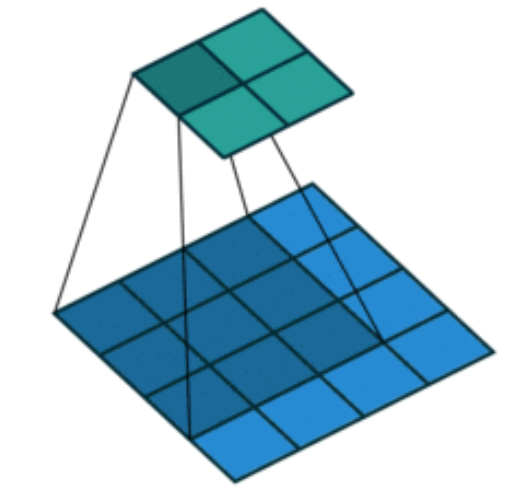
\includegraphics[width=0.42\textwidth]{figures/conv.png}} \qquad
	\subfloat[逆卷积操作]{\label{fig:dconv}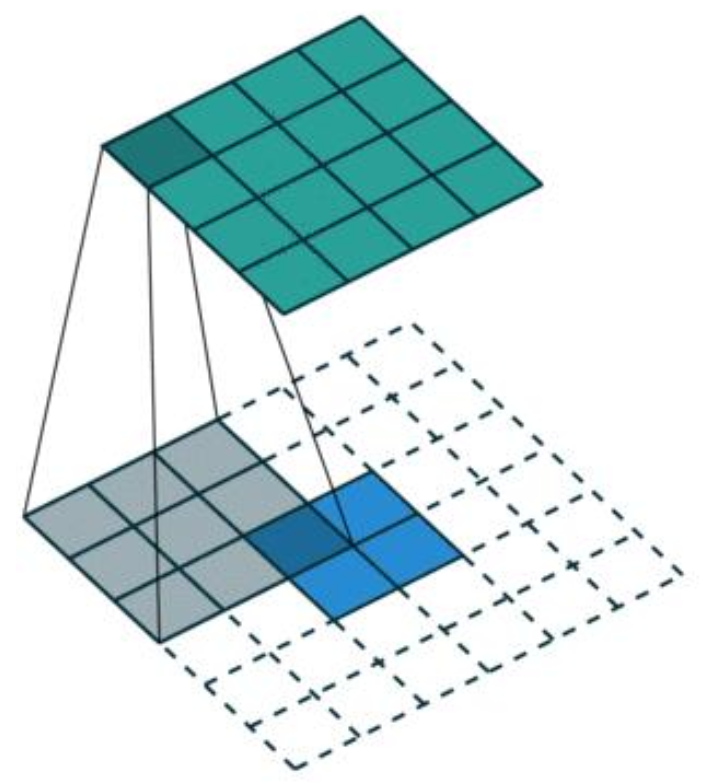
\includegraphics[width=0.38\textwidth]{figures/dconv.png}} 
	\caption{逆卷积操作原理}
	\label{fig:conv_dconv}
\end{figure}

%\begin{figure}[htp]
%	\centering
%	%\includegraphics[width=0.42\textwidth]{data/MLP.pdf}
%	subfigure[卷积操作]{\label{fig:conv}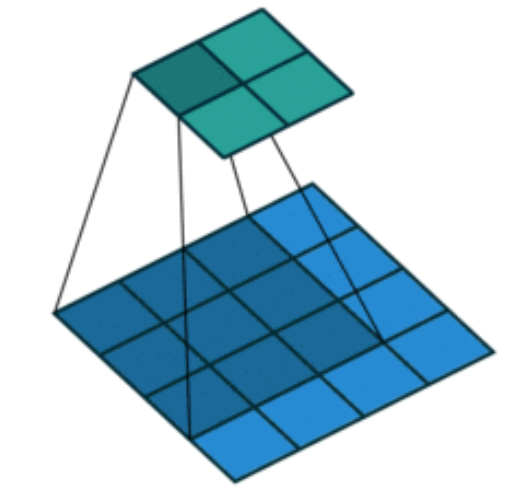
\includegraphics[width=0.42\textwidth]{figures/conv.png}}
%	subfigure[逆卷积操作]{\label{fig:dconv}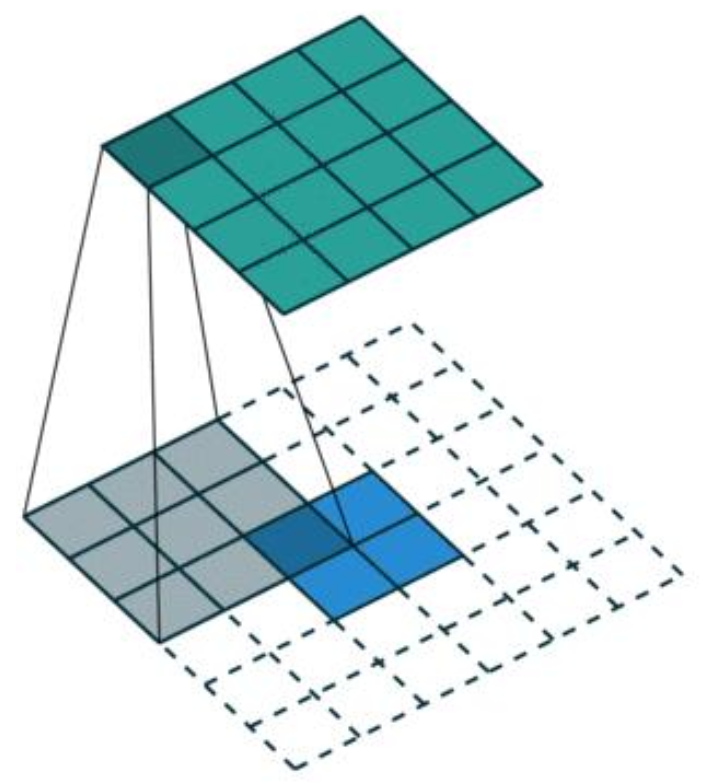
\includegraphics[width=0.42\textwidth]{figures/dconv.png}}
%	\caption{逆卷积操作原理}
%	\label{fig:conv_dconv}
%\end{figure}


对于无监督学习,在卷积神经网络的编码器和解码器的衔接处,利用全连接层,也可以提取带图像数据特征表示;在进行有监督学习时,网络更关注解码器的输出$Y^{\prime}$而不是z,损失函数转化为:
\begin{equation}
Loss_{MSE} = \min _{\phi, \theta}\left\|Y-Y^{\prime}\right\|_{2}^{2}
\end{equation}
从而可以利用卷积神经网络进行有监督学习任务,在气动流场模拟领域已有基于卷积自编码网络开展的工作\cite{DBLP:conf/kdd/GuoLI16}。



\subsection{基于深度学习的图像分割模型}
图像分割一直是计算机视觉领域的难题,也是该领域的研究热点。
图像分割是指根据图像灰度、色彩和外形等特征将图像进行区域划分,同区域中图像特征相似,而该特征又区别于其他区域\cite{图像分割方法综述}。

传统的图像分割技术有基于阈值的分割方法;基于区域和阈值的图像分割方法;基于小波分析和小波变换的分割方法;基于遗传算法的分割方法等。
随着深度学习技术的发展,基于深度学习的图像分割方法不断涌现,通过搭建深度神经网络对图像数据进行有监督学习,得到图形分割的模型。图像分割任务随着分割任务的难度逐渐增加可分为普通分割、语义分割和实例分割。其中:普通分割的任务对图像的每个像素点进行区域分类,任务相对简单为多分类任务;语义分割则需要是在像素点分类的基础上进一步识别出每一块区域的语义;实例分割任务对图像分割模型要求最高,需要在分类识别的基础上,对每个识别目标进行编号。本节重点介两种经典的语义分割网络:用于自然图像分割的全卷积网络和用于医疗图像分割的U-net网络。


\subsubsection{全卷积网络}
2015年Long等人提出的全卷积网络(Fully Convolutional Networks,FCN)用于图像语义分割\cite{Long2015Fully}。
FCN提出的编码-解码的思想,一直为之后图像分割网络模型所沿用。

\begin{figure}[htp]
	\centering
	%\includegraphics[width=0.42\textwidth]{data/MLP.pdf}
	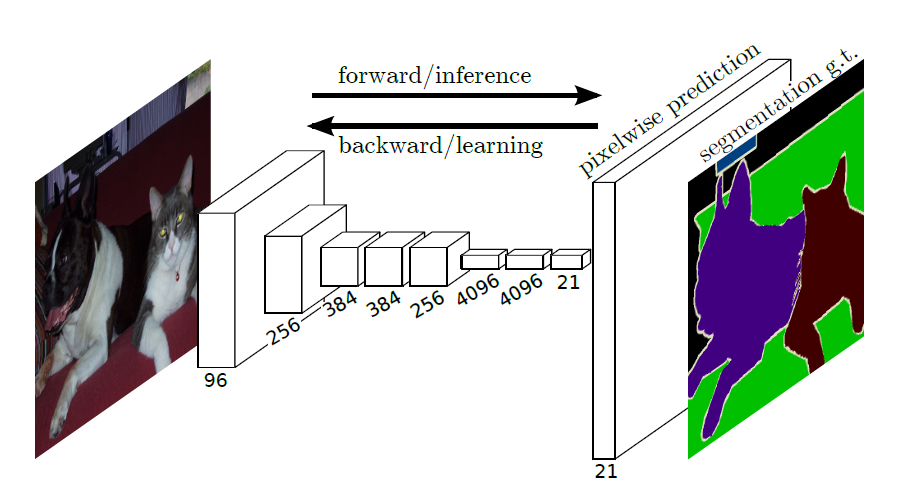
\includegraphics[width=0.88\textwidth]{figures/FCN.png}
	\caption{FCN网络结构图}
	\label{fig:FCN}
\end{figure}

如图\ref{fig:FCN}所示,FCN参考了图像分类网络中的VGG16\cite{2014Very}网络架构。图像分类网络只能对整个图片进行分类而不能识别每个像素点的类别。
因此FCN用卷积层替换了VGG网络中的全连接层实现了逐像素分类,最后利用逆卷积的上采样方法将特征图恢复成原始图片大小,从对整张图片的稀疏分类转换成对每个像素点进行密集分类(dense prediction),达到图像分割的目的。

FCN的另一个特点是利用了全局信息和局部信息。输入数据经过多个卷积层和池化层会导致输入特征图变小同时分辨率降低,最后产生了高维特征图。如果直接对进行上采样至原始图片大小,会产生模糊的分割结果。为了产生清晰的分割结果,FCN使用了如图\ref{fig:FCN_skip}所示的skip layer的方法。

以FCN-32s为例,高层得到的粗糙层(conv7)进行32倍上采样操作,再对每个点进行softmax逻辑回归处理,得到每一个像素点的分类。
通过skip layer的方法,融合多层特征图,有效整合了粗粒度的语义信息和细粒度的位置信息,有利于提高分割准确性。
尽管8倍上采样的FCN的分割效果已经有了很大提升,但是分割区域边界比较模糊;
此外,由于FCN网络只进行素点维度的分类任务,因此缺少对图像空间上局部信息的有效利用。

\begin{figure}[htp]
	\centering
	%\includegraphics[width=0.42\textwidth]{data/MLP.pdf}
	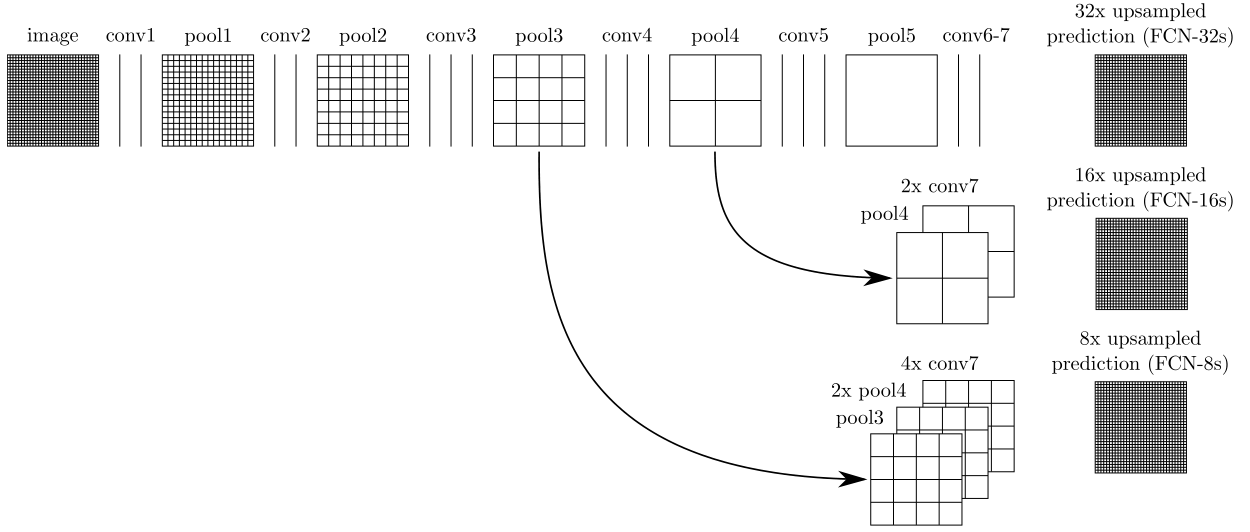
\includegraphics[width=0.88\textwidth]{figures/FCN_skip.png}
	\caption{FCN采用的skip layer方法}
	\label{fig:FCN_skip}
\end{figure}

\subsubsection{U-net网络}
2015年,Ronneberger等人\cite{DBLP:conf/miccai/RonnebergerFB15}针对医学图像的分割任务在FCN网络基础上提出了U-net网络结构,降低了精确分割结果对数据样本的要求。
其主要思想是在下采样网络的后面补充一个对称的上采样网络,多个上采样层增加了网络的参数和表示能力,有利于提升输出结果的分辨率。
图\ref{fig:unet}展示了U-net网络结构:
输入特征图信息经过卷积层进行特征提取,利用池化层降低维度,在编码过程中特征图大小逐渐减小;
在解码时,使用上采样层恢复维度,再利用卷积层对输出结果进行微调。连接编码部分和解码部分的灰色箭头代表跳跃连接(skip-connection)操作,连接浅层信息和深层信息。其中灰色箭头中的copy就是拼接操作,将深层的特征图和浅层的特征图在通道方向拼接;crop代表裁剪操作,是为了参与拼接的特征图的长宽一致,保证拼接后的特征图大小一致。


\begin{figure}[htp]
	\centering
	%\includegraphics[width=0.42\textwidth]{data/MLP.pdf}
	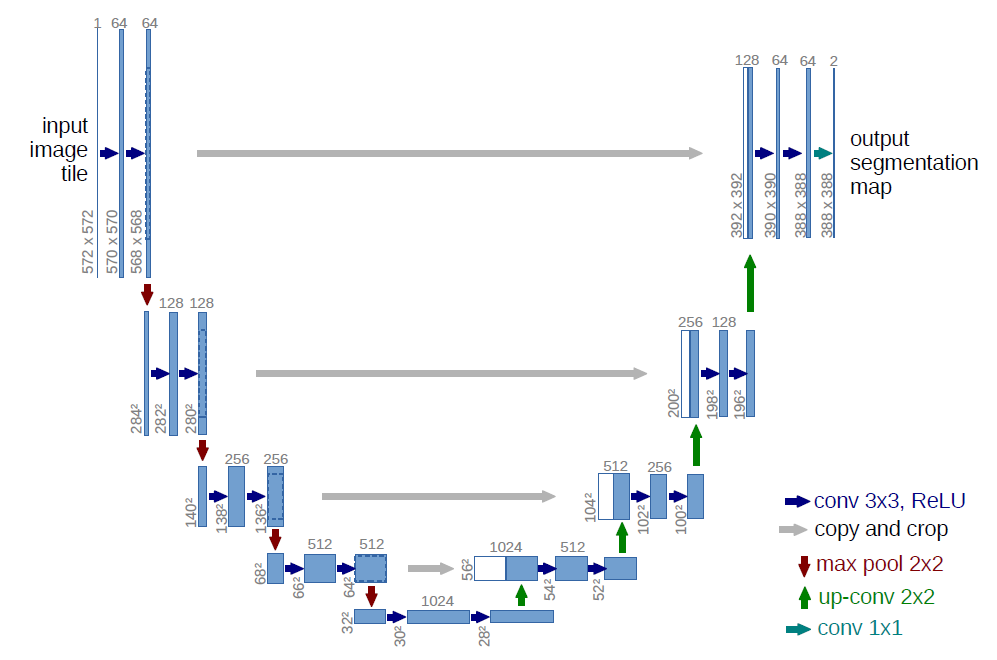
\includegraphics[width=0.88\textwidth]{figures/unet.png}
	\caption{U-net网络结构图\cite{DBLP:conf/miccai/RonnebergerFB15}}
	\label{fig:unet}
\end{figure}

U-net主体结构包括收缩路径部分和精确定位部分:
收缩部分和扩展部分都有4个采样层。这种架构延续了编码-解码的思想。
Encoder由卷积层和下采样层组成,为了保证卷积操作不改变特征图大小,使用3x3的卷积核,填充为 0,步长为1;Decoder部分采用的上采样的方式与FCN中的反卷积不同,为双线性插值。
此外,为了更好融合位置信息和语义信息,U-net拓展了FCN中skip layer的思想,在“U”形网络的对称部分添加了跳跃连接。与FCN的加操作不同,U-net使用了叠操作(concatenation)增加了特征的厚度而保留了更多的浅层位置信息,利用卷积层使网络自适应调整深层信息和浅层信息的权重从而增强网络的学习能力。

许多研究者针对不同的图像分割任务对U-net进行了改进,产生了许多U-net变体包括V-Net\cite{2016V}、UNet++\cite{unet++}、U-NetPlus\cite{unetplus}和3D U2-Net\cite{20193D}等,提升了模型的推理速度和精度。


\subsection{Pix2Pix网络模型}
对于气动流场预测,核心问题是获取从条件输入到流场模拟输出的映射函数。
除了前文提到的自编码网络和图像分割网络,基于生成对抗网络(Generative Adversarial Network, GAN)的图像风格迁移模型也在解决像素到像素的映射问题上展示出的强大潜力。
GAN已经广泛应用于在图像生成、风格迁移、超分辨重建等领域,
本节我们重点介绍Pix2Pix网络模型\cite{isola2017image}。

Pix2Pix网络基于条件生成对抗网络\cite{cGAN},通过添加条件约束信息来指导完成图像转换任务。
和传统的GAN网络类似,在Pix2Pix模型训练过程中,迭代地训练生成器和判别器,生成器尽可能生成接近真实的样本,企图“欺骗”判别器;判别器尽可能识别出真实的样本和生成的样本,获得更高的得分。这样的对抗训练过程类似博弈游戏,随着训练的进行,生成器和判别器的能力不断提升直到达到令人满意的效果。
Pix2Pix网络的输入是约束条件而不再是普通GAN网络中的随机变量,其网络结构示意图
如图\ref{fig:cgan}所示:

\begin{figure}[htp]
	\centering
	%\includegraphics[width=0.42\textwidth]{data/MLP.pdf}
	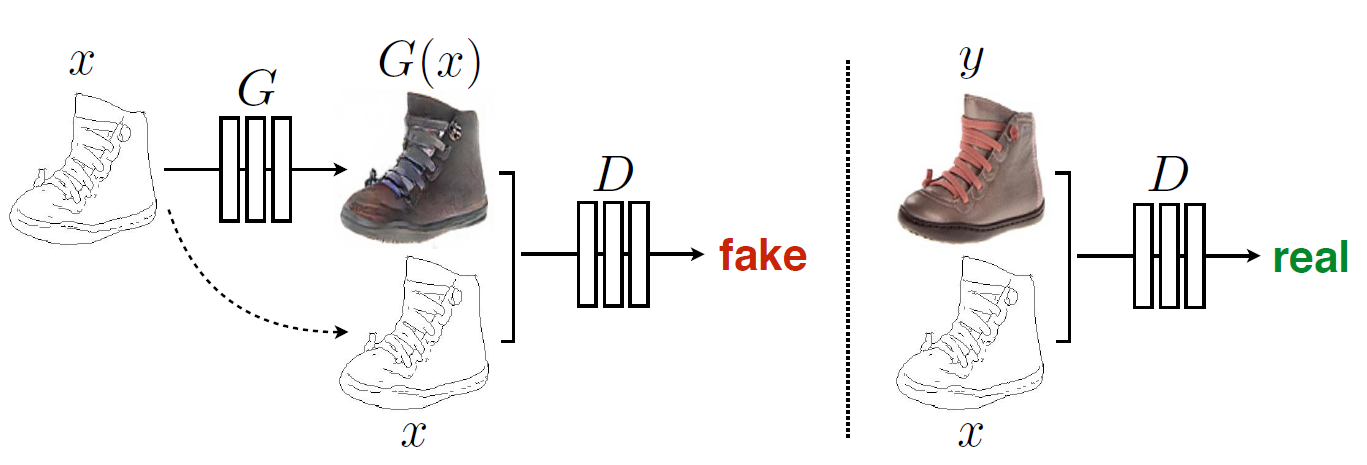
\includegraphics[width=0.88\textwidth]{figures/cGAN.png}
	\caption{Pix2Pix网络结构示意图}
	\label{fig:cgan}
\end{figure}

其中x是条件输入,y是对应的标签,每个输入x唯一对应一个标签y。
在训练生成器时,x进过生成器$G$得到生成图像$G(x)$;
在训练判别器时,输入x和对应生成图像$G(x)$或标签y通过通道维度的叠操作进行拼接,一同送入判别器,判别器会输出概率值,表示是否为一对真实样本。



Pix2Pix网络利用类似U-net的结构代替自编码网络作为生成器,因为采用skip-connection的结构有利于传递这些底层信息和重构图像。
对于判别器网络,Pix2Pix提出了PatchGAN架构。
传统GAN判别器通常对生成样本整体进行判断,比如进行图片生成时直接输出整张图片是真实样本的概率。而图像转换任务中关注像素到像素的转换效果,所以在这里提出了分块判断的算法,在图像的每个块上去判断是否为真,输出平均预测结果。


条件GAN采用的损失函数通常为:
\begin{equation}
\begin{aligned}
\mathcal{L}_{c G A N}(G, D)= &\mathbb{E}_{x,y}[\log D(x,y)]+\\
&\mathbb{E}_{x,z }[\log (1-D(x, G(x,z))]
\end{aligned}
\end{equation}

\begin{equation}
\begin{aligned}
\mathcal{L}_{c G A N}(G)= \mathbb{E}_{x,z}[\log (1-D(x, G(x, z))]
\end{aligned}
\end{equation}

\noindent 其中z为输入随机变量,在Pix2Pix网络输入仅为x。
此外,为了保证像素级低频信息的预测精度,Pix2Pix网络的损失函数还引入了$L_1$损失项:

\begin{equation}
\begin{aligned}
\mathcal{L}_{L 1}(G)=\mathbb{E}_{x_1, x_2, y}\left[\|y-G(x_1, x_2)\|_{1}\right]
\end{aligned}
\end{equation}

考虑到训练的最终目标是获得一个性能良好的生成器,同时生成器和判别器进行着对抗的训练,所以训练的最终目标是:
\begin{equation}
\begin{aligned}
G^{*}=\arg \min _{G} \max _{D} \mathcal{L}_{c G A N}(G, D)+\lambda \mathcal{L}_{L 1}(G)
\end{aligned}
\end{equation}
\noindent 其中$\lambda$是$L_1$损失函数项的权重系数。


\subsection{图卷积神经网络}

在深度学习发展过程中,卷积神经网络和循环神经网络在图像识别、语义分割、自然语言处理等领域发挥了重要作用。
无论是图像还是语言,通常都被转换成结构规则的数据形式,都属于欧式空间的数据。
然而生活中更常见的是非结构数据,如社交关系和生物网络等。
图结构通常被用来表示这些非欧式空间的数据,但是在图结构中,每个节点周围的结构千差万别,
不同于图像和向量化的语言数据具有平移不变性,因此不可能直接利用卷积神经网络或循环神经网络进行处理。

近年来,人们对深度学习方法在图上的拓展进行了大量的研究,类比卷积神经网络设计了专用于处理图结构数据的神经网络,
即图神经网络(Graph  Neural  Network, GNN)。
文献\cite{2019A}将GNN分为五大类:图卷积网络、 图注意力网络、图自编码器、图生成网络和图时空网络。
本节重点介绍图卷积网络。

GCN方法主要分为两大类,基于谱的GCN和基于空间的GCN。
前者利用傅里叶变换和傅里叶逆变换在频域中完成信号的分析处理,根据图谱理论和卷积定理,将数据由空域转换到谱域做处理,理论基础坚实。后者直接在图空间上定义卷积操作,每个图节点与相邻节点进行信息聚合,灵活性更强。
本章重点介绍基于谱的GCN的工作原理,
对于无向图有正则化拉普拉斯矩阵:

\begin{equation}
\mathbf{L}=\mathbf{I}_{\mathbf{n}}-\mathbf{D}^{-\frac{1}{2}} \mathbf{A} \mathbf{D}^{-\frac{1}{2}}
\end{equation}

\noindent $I_n$为单位矩阵,A为图的邻接矩阵,D为对角矩阵。
对L进行特征值分解有:

\begin{equation}
\mathbf{L}=\mathbf{U} \mathbf{\Lambda} \mathbf{U}^{T}
\end{equation}

\noindent U是特征向量构成的矩阵,$\Lambda$是对角矩阵,对角线上的值为L的特征值。
对输入图信号x的傅里叶变换和傅里叶逆变换分别被定义为

\begin{equation}
\mathfrak{F}(\mathrm{x})=\mathbf{U}^{T} \mathrm{x} 
\end{equation}
\begin{equation}
\mathfrak{F}^{-1}(\hat{\mathrm{x}})=\mathbf{U} \hat{\mathrm{x}}
\end{equation}

\noindent $\hat{\mathrm{x}}$为傅里叶变换的结果。
图卷积操作可被定义为:

\begin{equation}
\begin{aligned}
\mathrm{x} *_{G} \mathrm{g} &=\mathfrak{F}^{-1}(\mathfrak{F}(\mathrm{x}) \odot \mathfrak{F}(\mathrm{g})) \\
&=\mathbf{U}\left(\mathbf{U}^{T} \mathrm{x} \odot \mathbf{U}^{T} \mathrm{g}\right)
\end{aligned}
\end{equation}
\noindent 其中g是定义的滤波器,$\odot$表示哈达玛积运算。
一直以来研究人员不断探索和尝试不同的滤波器,增强基于谱方法的图卷积网络的表示能力。





\begin{figure}[htp]
	\centering
	%\includegraphics[width=0.42\textwidth]{data/MLP.pdf}
	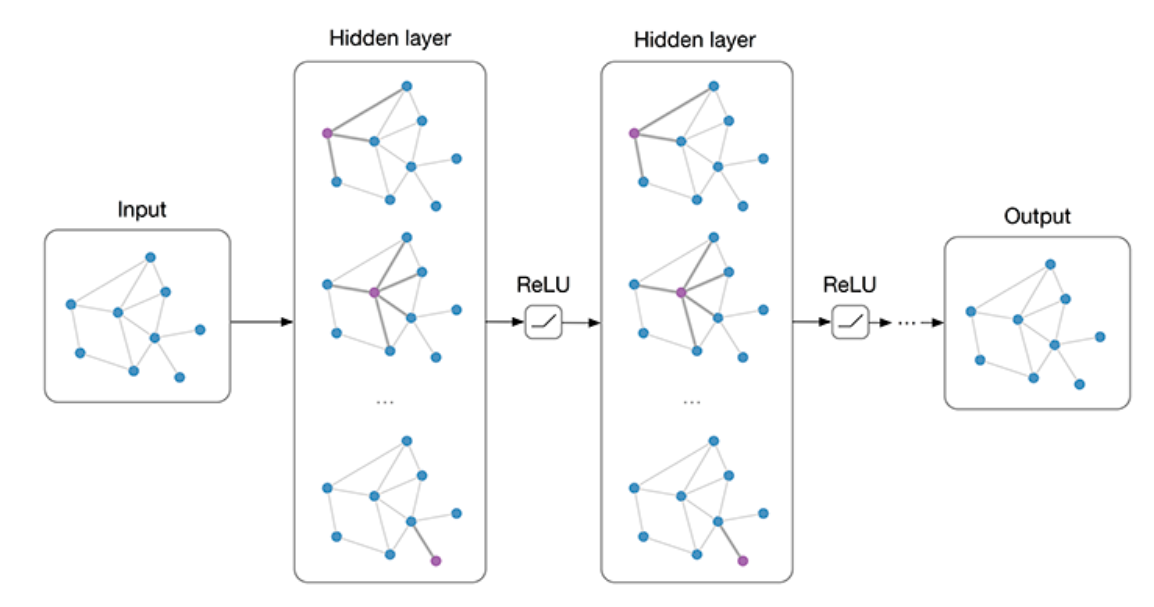
\includegraphics[width=0.88\textwidth]{figures/GCN.png}
	\caption{多层GCN网络示意图}
	\label{fig:gcn}
\end{figure}

对于图卷积算法的实现主要包括三个步骤:
\romannumeral1)发送:每个节点与相邻节点进行通信发送自身节点特征信息,达到提取变换特征信息的效果;
\romannumeral2)接收:每个节点接受并整合相邻节点发送的信息,实现局部信息的交换与融合;
\romannumeral3)变换:非线性激活函数对整合的信息进行再处理,增强模型的非线性,。
图\ref{fig:gcn}展示了一个简单的GCN网络,从图中可以发现图拓扑结构在训练过程中始终保持不变,
可以在训练中重复利用。
每一层的节点特征维度是不固定的,可以根据训练任务的复杂程度进行灵活的调整。

概括而言,图卷积算子的作用是聚合周围节点的特征信息并传播到下一层,具有以下特点:
1)局部参数共享,计算节点特征值时,按一定规律将参与聚合的节点分为若干个子集,
同一个子集内的节点采用相同的权重;
2)节点感受域正比于层数,每一层图卷积运算只能和相邻的节点进行特征聚合;通过增加GCN层数,可以扩大图节点信息交换的范围,使图节点计算利用更多信息;
3)具有通用性,对图结构没有特殊要求,基于节点特征信息和图拓扑结构可以实现对图数据的表示与学习。


%\section{实验算例介绍}
%\subsection{2D不可压层流固体外部流场}
%\subsection{2D不可压有粘翼型外部流场}



\section{本章小结}

本章首先通过对比传统CFD求解器和基于深度学习的气动优化模型的工作流程,明确了利用深度学习技术和方法要解决的CFD问题。
然后介绍了CFD相关理论知识,重点介绍了在宏观和介观层面对流体运动规律的描述。
最后分析了气动流场模拟任务和深度学习中图像回归预测任务的相似性,介绍了与本文研究内容紧密相关的深度网络模型。





